%# -*- coding:utf-8 -*-
\documentclass[10pt,aspectratio=169,mathserif]{beamer}		
%设置为 Beamer 文档类型,设置字体为 10pt,长宽比为16:9,数学字体为 serif 风格

%%%%-----导入宏包-----%%%%
\usepackage{CSU}			%导入 CSU 模板宏包
\usepackage{ctex}			%导入 ctex 宏包,添加中文支持
\usepackage{xeCJK}
\usepackage{amsmath,amsfonts,amssymb,bm}   %导入数学公式所需宏包
\usepackage{color}			 %字体颜色支持
\usepackage{graphicx,hyperref,url}
\usepackage{metalogo}	% 非必须
\usepackage{booktabs}   %提供表格命令\toprule、\midrule、\bottomrule
\usepackage[backend=biber,style=gb7714-2015]{biblatex}
\usepackage{mhchem}    %化学方程式支持
%% 上文引用的包可按实际情况自行增删
%%%%%%%%%%%%%%%%%%	
% 设置字体
\setsansfont{Helvetica} 							%Windows和Mac OS下都可用

%\setCJKmainfont{Microsoft YaHei}   	%仅Windows可用
\setCJKmainfont{Songti SC}								%仅Mac OS下可用

\beamertemplateballitem		%设置 Beamer 主题
%%%%------------------------%%%%%
%在章节首是否需要再显示一遍加粗的默认页,本示例中未显示。
%\AtBeginSection[]
%{\begin{frame}<beamer>
%		\frametitle{\textbf{目录}}
%		\textbf{\tableofcontents[currentsection]}
%	\end{frame}}
%%%%------------------------%%%%%
\catcode`\。=\active         %或者=13
\newcommand{。}{.}				
%将正文中的“。”号转换为“.”。中文标点国家规范建议科技文献中的句号用圆点替代
%%%%%%%%%%%%%%%%%%%%%

%%%%----首页信息设置----%%%%
\title{\lishu{中南大学 Beamer 的模板}}
\subtitle{——这里是副标题}			
%%%%----标题设置


\author{
  HMPA \\\medskip
  {\small \url{Hexa_mpa@tom.com}} \\
  {\small \url{http://www.csu.edu.cn/}}}
%%%%----个人信息设置
  
\institute{\small
  化学化工学院 \\\smallskip
  中南大学}
%%%%----机构信息

\date{
  \today}
%%%%----日期信息
\addbibresource{thesis.bib}
%%%%----参考文献
\begin{document}

\begin{frame}
\titlepage
\end{frame}				%生成标题页

\section*{目录}
\begin{frame}
\frametitle{目录}
\centering
\textbf{\tableofcontents}


\end{frame}				%生成目录页

\section{介绍}
\begin{frame}
  \frametitle{介绍}

  \begin{itemize}
    \item {编译方式}
	    \begin{itemize}
	    	\item  本文档在Miktex 2.9下编译通过
	    	\item 使用 \XeLaTeX 编译
	    \end{itemize}
    \item 请参考 \LaTeX 和 Beamer 用户文档 
    
    \item 行内数学公式示例 $\sin^2 \theta + \cos^2 \theta = 1$
    \item {行间数学公式示例 \begin{equation}
	    y_{1}=\int \sin x\, {\rm d}x
    \end{equation}	 }   
    \item 基于“中南蓝”颜色 \url{http://www.csu.edu.cn/}
    \item 待续
  \end{itemize}
\end{frame}

\section{内置环境}
\begin{frame}
  \frametitle{内置环境}
	\begin{block}{用 \LaTeX 做幻灯片}
	    Beamer 提供了很多功能来使用\LaTeX 创建漂亮的幻灯片。
	    
	  \end{block}
	
	  \begin{block}{基础}
	    内部使用以下主题
	    \begin{itemize}
	      \item split
	      \item whale
	      \item rounded
	      \item orchid
	    \end{itemize}
	  \end{block}
\end{frame}

\begin{frame}
  \frametitle{带数字列表}
	 \begin{enumerate}
	    \item 这只是显示样式的效果
	    \item 这不是 Beamer 教程
	    \item 阅读 Beamer 手册以获得更多帮助
	    \item 仅就样式文件与我联系 
	  \end{enumerate}
\end{frame}

\begin{frame}
	\frametitle{公式}
	这里有举一个长公式排版的例子,来自\href{http://www.tex.ac.uk/tex-archive/info/math/voss/mathmode/Mathmode.pdf}{《Math mode》}:
	
	\begin{multline}
		\frac {1}{2}\Delta (f_{ij}f^{ij})=
		2\left (\sum _{i<j}\chi _{ij}(\sigma _{i}-
		\sigma _{j}) ^{2}+ f^{ij}\nabla _{j}\nabla _{i}(\Delta f)+\right .\\
		\left .+\nabla _{k}f_{ij}\nabla ^{k}f^{ij}+
		f^{ij}f^{k}\left [2\nabla _{i}R_{jk}-
		\nabla _{k}R_{ij}\right ]\vphantom {\sum _{i<j}}\right )
	\end{multline}
还有一个化学方程式的例子
\begin{equation}
	\ce{Zn^2+  <=>[+ 2OH-][+ 2H+]  $\underset{\text{amphoteres Hydroxid}}{\ce{Zn(OH)2 v}}$  <=>[+ 2OH-][+ 2H+]  $\underset{\text{Hydroxozikat}}{\ce{[Zn(OH)4]^2-}}$} 	
\end{equation}

\end{frame}
\begin{frame}
	\frametitle{图文混排}
		\begin{columns}
			\column{.5\textwidth}
			\normalsize
			\XeTeX 可以很方便地插入PDF、PNG、JPG格式的图片。这里还有插入EPS图像和PDF图像的例子,如图,这里将EPS和PDF图片作为子图插入,每个子图有自己的小标题。子图标题使用subcaption宏包添加。
			\column{.5\textwidth}
			\begin{figure}[!htp]
				\centering
				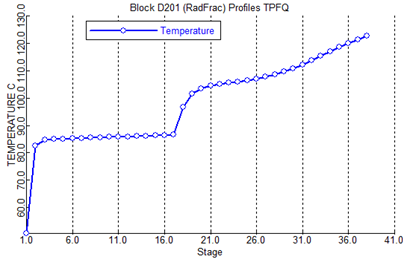
\includegraphics[scale=0.5]{res/tem.png}
				\caption{塔板温度分布图}
				\label{fig:tem}
			\end{figure}
		\end{columns}
\end{frame}

\begin{frame}
	\frametitle{文表混排}
	\begin{columns}
		\column{.4\textwidth}
		\normalsize
		这一节给出的是一些表格的例子,如表\ref{tab:firstone}所示。
		\column{.6\textwidth}
		\begin{table}[!htpb]
			\caption{一个颇为标准的三线表格}
			\label{tab:firstone}
			\begin{tabular}{@{}llr@{}} \toprule
				\multicolumn{2}{c}{Item} \\ \cmidrule(r){1-2}
				Animal & Description & Price (\$)\\ \midrule
				Gnat & per gram & 13.65 \\
				& each & 0.01 \\
				Gnu & stuffed & 92.50 \\
				Emu & stuffed & 33.33 \\
				Armadillo & frozen & 8.99 \\ \bottomrule
			\end{tabular}
		\end{table}
	\end{columns}
\end{frame}

\begin{frame}{引用}
	按照教务处的要求,参考文献外观应符合国标GBT7714的要求\footnote{\url{http://www.cces.net.cn/guild/sites/tmxb/Files/19798_2.pdf}}。
	在模板中,表现形式的控制逻辑通过biblatex-gb7714-2015包实现\footnote{\url{https://www.ctan.org/pkg/biblatex-gb7714-2015}},基于{Bib\LaTeX}管理文献。在目前的多数TeX发行版中,可能都没有默认包含biblatex-gb7714-2015,需要手动安装。\\
	正文中引用参考文献时,可以用cite命令产生“上标引用的参考文献”,也可以parencite命令产生“正常标引用的参考文献”,如\cite{Meta_CN,chen2007act,DPMG}。关于期刊的\cite{chen2007act,chen2007ewi},
	会议论文\parencite{DPMG,kocher99,cnproceed},
	硕士学位论文\parencite{zhubajie,metamori2004}等等。\\
	总结一些注意事项:
	\begin{itemize}
		\item 参考文献只有在正文中被引用了,才会在最后的参考文献列表中出现;
		\item 参考文献“数据库文件”bib是纯文本文件,请使用UTF-8编码,不要使用GBK编码;
		\item 参考文献条目中默认通过date域输入时间。兼容使用year域时会产生编译warning,可忽略。
	\end{itemize}
\end{frame}

\section{结论}
\begin{frame}
	\frametitle{结论}
	
	\begin{itemize}
		\item Easy to use
		\item Good results
	\end{itemize}
\end{frame}
\begin{frame}{参考文献}
	\printbibliography
\end{frame}

\begin{frame}{参考文献}
\begin{thebibliography}{99} 
\bibitem{zhao1} Yi~Zhao, {\sl An introduction to X}, Sep.~15, 2015
\bibitem{qian2} Er~Qian, San~Sun, 
Phys.\ Lett.\ A {\bf xx}, 2xx (20xx)   
\bibitem{li4} Si~Li, Phys.\ Rev.\ C {\bf xx}, 5xx (20xx) 

\end{thebibliography}
\end{frame}


\section*{结束页}
\begin{frame}
	
	\begin{center}
		\begin{minipage}{1\textwidth}
			\begin{beamercolorbox}[wd=0.70\textwidth, rounded=true, shadow=true]{subsection in head/foot}
				\LARGE \centering Thanks for Listening.
			\end{beamercolorbox}
		\end{minipage}
	\end{center}
	
	
\end{frame}
\end{document}